\documentclass[10pt, conference]{IEEEtran}
\usepackage{cite}
\usepackage{amsmath,amssymb,amsfonts}
\usepackage{algorithmic}
\usepackage{graphicx}
\usepackage{textcomp}
\usepackage{balance}
\usepackage{comment}
\usepackage[group-separator={,}]{siunitx}
\usepackage{grffile}
\usepackage{subcaption}
\usepackage{lipsum}
\usepackage{float}


\usepackage[T1]{fontenc}
\def\BibTeX{{\rm B\kern-.05em{\sc i\kern-.025em b}\kern-.08em
    T\kern-.1667em\lower.7ex\hbox{E}\kern-.125emX}}

%%%%%%%%%%%%%%%%% Macros %%%%%%%%%%%%%%%%%

\newcommand{\vectorScheme}{\textit{Vector Scheme}}
\newcommand{\valueScheme}{\textit{Value Scheme}}
\newcommand{\distanceScheme}{\textit{Distance Scheme}}
\newcommand{\distanceLemma}{\textit{Distance Lemma}}
\newcommand{\sketchScheme}{\textit{Sketched Data Scheme}}
\newcommand{\fullSync}{\textit{Full Sync}}
\newcommand{\naiveScheme}{\textit{Naive Scheme}}
\newcommand{\oracleScheme}{\textit{Oracle Scheme}}
\newcommand{\falseAlarm}{\textit{false alarm}}
\newcommand{\falseAlarms}{\textit{false alarms}}
\newcommand{\coveringSpheres}{\textit{Covering Spheres}}
\newcommand{\convexDecomposition}{\textit{Convex Decomposition}}
\newcommand{\convexBound}{\textit{Convex Bound}}
\newcommand{\theCoordinator}{\textit{the coordinator}}
\newcommand{\Coordinator}{\textit{Coordinator}}
\newcommand{\TheCoordinator}{\textit{The coordinator}}
\newcommand{\safeZone}{\textit{safe zone}}

%%%%%%%%%%%%%%%%% Document %%%%%%%%%%%%%%%%%
\begin{document}

%%%%%%%%%%%%%%%%% Title %%%%%%%%%%%%%%%%%
\title{Guaranteed Approximation and Bandwidth Efficient Distributed Function Monitoring Schemes}
\author{
\begin{tabular}{c c c}
Yuval Alfassi & Dani Keren & Moshe Gabel \\
\textit{Computer Science Department} & \textit{Computer Science Department} & \textit{Computer Science Faculty} \\
\textit{University of Haifa} & \textit{University of Haifa} & \textit{Technion} \\
Haifa, Israel & Haifa, Israel & Haifa, Israel \\
yuvalalfassi@gmail.com & dkeren@cs.haifa.ac.il & mgabel@cs.technion.ac.il\\
\ & \ & \ 
\end{tabular} \\
\begin{tabular}{c c c}
Assaf Shuster & \ \ \ \ & Gal Yehuda \\
\textit{Computer Science Faculty} & \ \ \ \ & \textit{Computer Science Faculty} \\
\textit{Technion} & \ \ \ \ & \textit{Technion} \\
Haifa, Israel & \ \ \ \ & Haifa, Israel \\
assaf@cs.technion.ac.il & \ \ \ \ & gal2016@gmail.com \\
\ & \ \ \ \ & \ 
\end{tabular}
}
\maketitle

%%%%%%%%%%%%%%%%% Abstract %%%%%%%%%%%%%%%%%
\begin{small}
\textbf{
\textit{Abstract}--- Distributed monitoring is a problem that arises when trying to monitor properties of dynamic data which is spread distributively. Tracking the value of a function over dynamic data in a distributed setting is a challenging problem in numerous real-world modern applications. Several monitoring schemes were proposed as an approach to coping with this problem in order to reduce the amount of communication messages between servers, as well as the communication bandwidth. \\
Here, we propose several new distributed monitoring schemes using much less communication bandwidth. Existing schemes send high dimensional vectors from server to server while we propose some innovative methods for reducing the dimensionality of the transmitted data even down to one single scalar.\\
One scheme we propose is the \valueScheme \ which exploits some traits of convex functions, and another is the \distanceScheme \ which treats the function monitoring problem as a geometric monitoring problem, thereby utilizing geometric distances for distributed monitoring. \\
Moreover, we present a clever way to incorporate lossy data-sketches into the schemes, which influence the bandwidth as well.}
\end{small}

%%%%%%%%%%%%%%%%% Introduction %%%%%%%%%%%%%%%%%
\section{Introduction}
Monitoring a function over large amount of dynamically changed data in a distributed fashion is a common computer-science challenge. Whether it's monitoring features of distributed sensor networks \cite{burdakis2012detecting}, top-k monitoring \cite{babcock2003distributed}, monitoring distributed ratio queries \cite{gupta2013ratio} or tracking properties of large distributed dynamic graphs \cite{mcgregor2015densest}, innovative approaches had to be developed in order to deal with the difficulties of both the data being dynamic and distributed. \\
The need of minimizing both the bandwidth and the processing power is expressed in \cite{giatrakos2013network}; a good example is internet of things objects which are operated on batteries, hence sending data via a communication channel should be minimized [*]. Furthermore, in the \textit{Big Data} era, where data is of very high dimensionality and changes rapidly, data transmition over a communication channel has to be planned cleverly. Transmition of high dimensional data is not only impractical, but also extremely time consuming; for instance, air pollution sensors which distributively have to determine the air pollution level may benefit from an economical communication approach \cite{cheng2004revised}. \\
Previous works were made on tracking the distributed value of linear functions \cite{keralapura2006communication}, where the linear properties make the distributed monitoring much easier; though, in order to monitor non-linear functions, a handful of difficulties arise. Works were done on distributively monitoring the entropy of distributed streams \cite{gabel2017anarchists}\cite{cormode2013continuous}, monitoring the inner-product value of distributed dynamic vectors \cite{garofalakis2013sketch}, monitoring distributevely least squares models \cite{gabel2015monitoring}, and monitoring the number of triangles of dynamic graphs held in distributed servers \cite{yehuda2017monitoring}. \\
It should be noted that the classic approach to distributed monitoring is the "periodic polling" technique \cite{cormode2013continuous} where the central server -- \theCoordinator , polls the distributed data-servers for their observation at a certain frequency. This method may miss peaks of critical global data-changes, and also may be more expensive communication-wise -- high dimensional data is transmitted even when the changes are small. \\
\subsection{Problem Definition}
Commonly, distributed monitoring schemes are focused on determining whether a function over dynamic distributed data crosses a certain threshold. This is used as a component to the \textit{distributed function approximation problem} \cite{garofalakis2013sketch}, which $\varepsilon$-approximates the value of a function over time. \\
The distributed model is described as follows:
\begin{enumerate}
\item There are $n$ data-servers, $server_1 ... server_n$
\item A central \textit{coordinator} exists, with whom the servers communicate.
\item $Server_i$ knows only its dynamic \textit{local vector} $v_i$. \\
\item The \textit{global vector} $v$ is the average of the local vectors:
\begin{equation}
v = \frac{1}{n}\sum\limits_{i=1}^n {v_i}
\end{equation}
\item A function $f$ is monitored over the \textit{global vector} $v$ so it's $\varepsilon$-approximated with 100\% confidence: let the estimation be the dynamic value $\mu$ (without loss of generality, assume ${\mu \geq 0}$), then at all times: 
\begin{equation}
(1-\varepsilon )\mu \leq f(v) \leq (1+\varepsilon )\mu
\end{equation}
\end{enumerate}
The \textit{threshold monitoring problem} \cite{garofalakis2013sketch}  monitors whether the function's value crosses a certain threshold. The function approximation problem is commonly reduces to two simultaneous threshold monitoring problems: let ${T = (1+\varepsilon )\mu}$ be the upper-bound threshold's value, then, the upper-bound monitoring objective is to determine whether:
\begin{equation}
f(v) \leq T
\end{equation}
Likewise, the lower-bound function monitoring is done with the threshold ${(1-\varepsilon )\mu}$. \\
In turn, this threshold monitoring can be treated as a \textit{geometric monitoring problem} \cite{sharfman2007geometric}, where one tries to find a \safeZone \ of vectors ${\{v \ | \ f(v) \leq T\}}$, which is a convex, so every linear combination of vectors inside this \safeZone \ is also inside the \safeZone , see Fig. \ref{fig:ConvexSafeZoneSketch}. This geometric \safeZone \ approach is the fundamental idea behind previous distributed monitoring techniques.
\begin{figure}[h]
\begin{center}
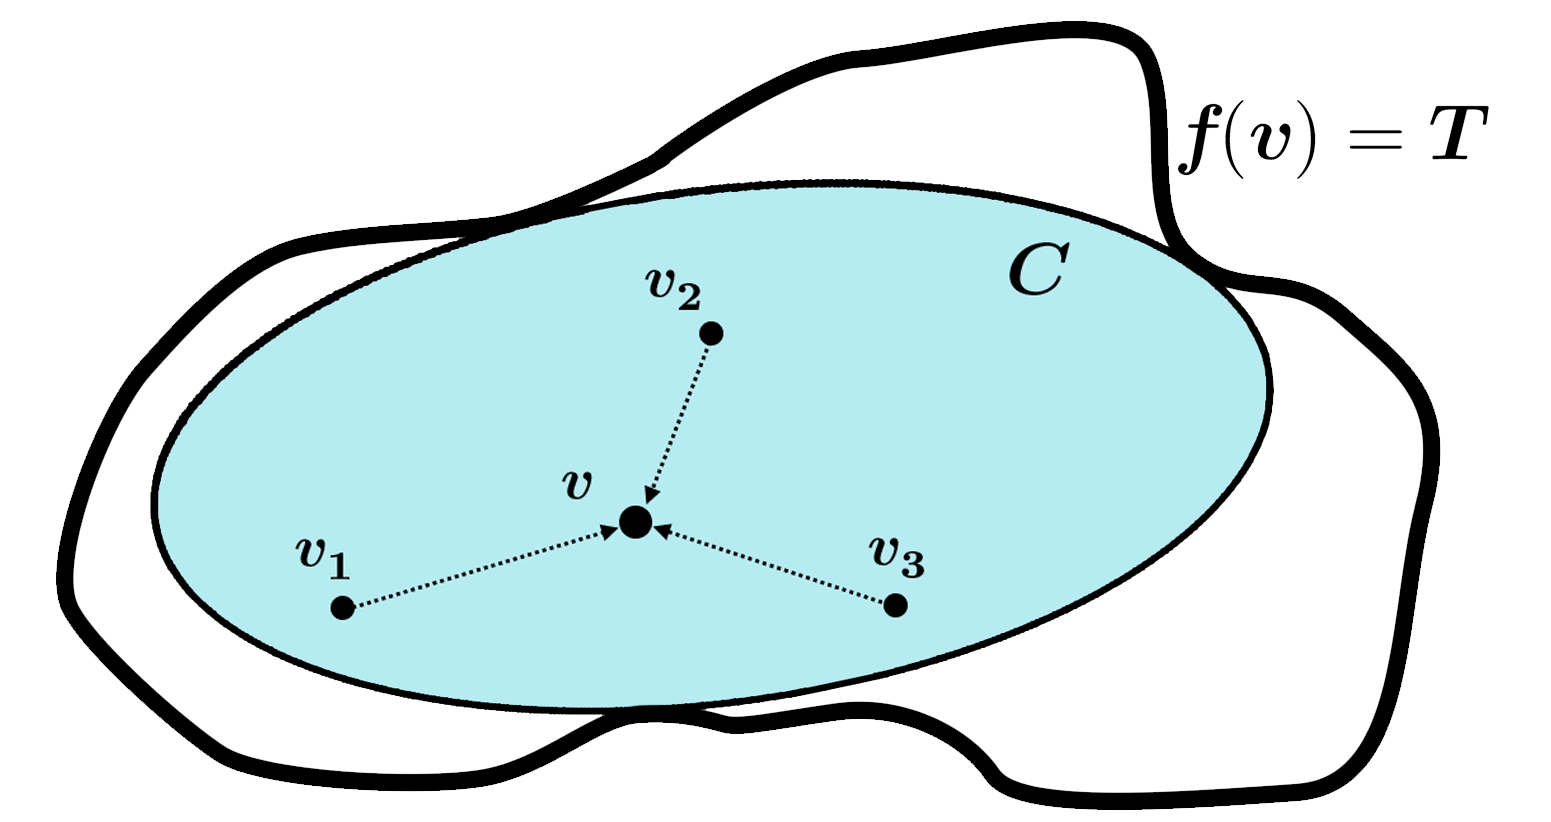
\includegraphics[width=0.85\linewidth]{Pics/PNGs/ConvexSafeZone.png}
\end{center}
\caption{Convex Safe Zone}
\label{fig:ConvexSafeZoneSketch}
\medskip
\small
$C$ is a convex subspace of ${\{v \ | \ f(v) \leq T\}}$ so since ${v_1,v_2,v_3 \in C}$, so does the average vector $v \in C$.
\end{figure}
\subsection{Distributed Monitoring Initiation}
When initiating the protocol of the distributed monitoring scheme, its often assumed the initial global vector $v$ is known to \theCoordinator \ as well to the local servers. In order to eliminate bias toward a certain server and to prevent local violations initially \cite{sharfman2007geometric},  the local vectors refer to the initial global vector $v$ as their \textit{reference vector}, noted by $r_0$: the monitoring is done so the servers doesn't operate on their local data vector but the reference vector plus their local dynamic data-change. Since at all times the global vector is still the average of the local vectors, this step is permitted. Note the change vectors as ${ch_1 ... ch_n}$, then: \\
\begin{equation}
v = \frac{v_1+...+ v_n}{n} = \frac{(r_0+ch_1)+...+(r_0+ch_n)}{n}
\end{equation}
So the local vector $server_i$ maintains the vector $v_i = r_0 + ch_i$ instead of the real data-vector. \\
A \textit{monitoring violation} occurs when a local server suspects that due to the current local change vector the function approximation or the threshold condition may not hold anymore -- so either this suspicion is true, and a \textit{true violation} occurs, so a \fullSync \ has to be invoked, or this was a \falseAlarm \ and a violation resolution protocol has to be done according to the distributed monitoring scheme. \\
The \fullSync \ gathers the whole data changes from the servers, recomputes the global average vector $v$, and transmits it to the servers so they set it to be their new reference point, while zeroing out the change vectors. In addition, the function's approximation is reset to the current value of $f(v)$ (since $v$ is known), and the lower-bound and upper-bound thresholds of the monitoring are set to ${(1 \pm \varepsilon )f(v)}$. \\
The communication channel is used when a local violation takes place; bandwidth is specifically wasted when \falseAlarms \ occur. Consequently, the distributed monitoring schemes we propose decrease the dimensionality of the transmitted data when a \falseAlarm \ takes place, in regard to the quantity of the occurrences of the \falseAlarms \ of the protocol.
\subsection{Contributions}
\begin{enumerate}
\item Introducing multiple innovative distributed monitoring schemes which avoid sending big dimensional data unless its crucially needed.
\item Proving the \distanceLemma , a lemma used as a basis of a distributed monitoring scheme we present. The \distanceLemma \ states that given a convex body and several points, if the sum of distances to the convex border from the points inside the convex body is greater than the sum of distances to the border from the points on the outside, then the average of the points is inside the convex body.
\item Incorporating data-sketches into distributed monitoring schemes without damaging the 0\% false-negative necessity of the distributed monitoring problem; i.e., we managed to prevent having the probabilistic nature of the sketches affect the distributed monitoring having a false-positive result.
\item Conducting several experiments, laying out comparisons of multiple attributes of distributed monitoring schemes on real-world data, focusing on the bandwidth consumption.
\end{enumerate}

%%%%%%%%%%%%%%%%% Previous Work %%%%%%%%%%%%%%%%%
\section{Previous Work}
\subsection{Linear Functions}
Since linear functions are additive and homogeneous, the basic algorithm for distributively monitoring their value is fairly easy. Since ${f(v) = \frac{1}{n}\sum f(v_i)}$, tracking the value of the global $f(v)$ isn't quite complicated. A work about linear functions such as the distributed count problem was done at \cite{keralapura2006communication}. However, things get more sophisticated when dealing with non-linear functions.
\subsection{The Covering Spheres Method}
The first approach which exploited some geometric traits of the ditributed monitoring problem is the \coveringSpheres \ method \cite{sharfman2007geometric}. This method is based on constraints on the local change-vectors. \\
Let $r_0$ be the reference point of the servers and $ch_i$ the change vector of $server_i$. Then, $server_i$ stays quiet if the sphere whose diameter is the segment between $r_0$ and $ch_i$ is fully inside the space ${\{v \ | \ f(v) \leq T\}}$. Turns out, this method artificially creates a convex safe zone subspace (as shown in Fig. \ref{fig:ConvexSafeZoneSketch}) where change vectors could be at without a need for communication. \\
This method seemed very effective theoratically, though it proved to be impractical. The \coveringSpheres \ method demands performing lots of time consuming heavy mathematical operations, so it isn't scalable computation-wise; moreover, this method requires computing distances to a high dimensional complicated surface, which does not have a closed mathematical solution nor a good approximation \cite{lazerson2018lightweight}. \\
Furthermore, the violation resolution phase demands transmitting high dimensional vectors, which makes the communication bandwidth quite too high.
\subsection{The Convex Decomposition Method}
Another distributed monitoring scheme previously developed is the \convexDecomposition \ method \cite{lazerson2015monitoring}. This method also treats the function monitoring problem as a geometric monitoring problem. The \convexDecomposition \ composes a convex \safeZone \ by decomposing the space ${\{v \ | \ f(v) \leq T\}}$ into convex subspaces and geometrically monitoring whether the average global vector is in their intersection. \\
Unfortunately, this method suffers from similar issues as the \coveringSpheres \ method, and cannot be applied on some basic functions, thus isn't feasable \cite{lazerson2018lightweight}
\subsection{The Convex Bound Method -- The Vector Scheme}
The \coveringSpheres \ method and the \convexDecomposition \ method turned out to be impractical albeit their mathematical purity. In need of more computationally lightweight and consistent monitoring approach, the \convexBound \ method was proposed \cite{lazerson2018lightweight}. \\
The \convexBound \ method simply bounds the monitored function by a convex function, so the convex bound serves as the convex safe zone: when monitoring $f(v) \leq T$, an upper bound convex $c$ has to be found so for all $v$, $f(v) \leq  c(v)$. \\
And the new monitoring objective becomes:
\begin{equation}
\label{monitoringConstraint}
c(v) \leq T
\end{equation}
The same goes for lower bound threshold monitoring -- It's done by bounding $f$ from below by a concave function.
\begin{figure}[t]
\begin{center}
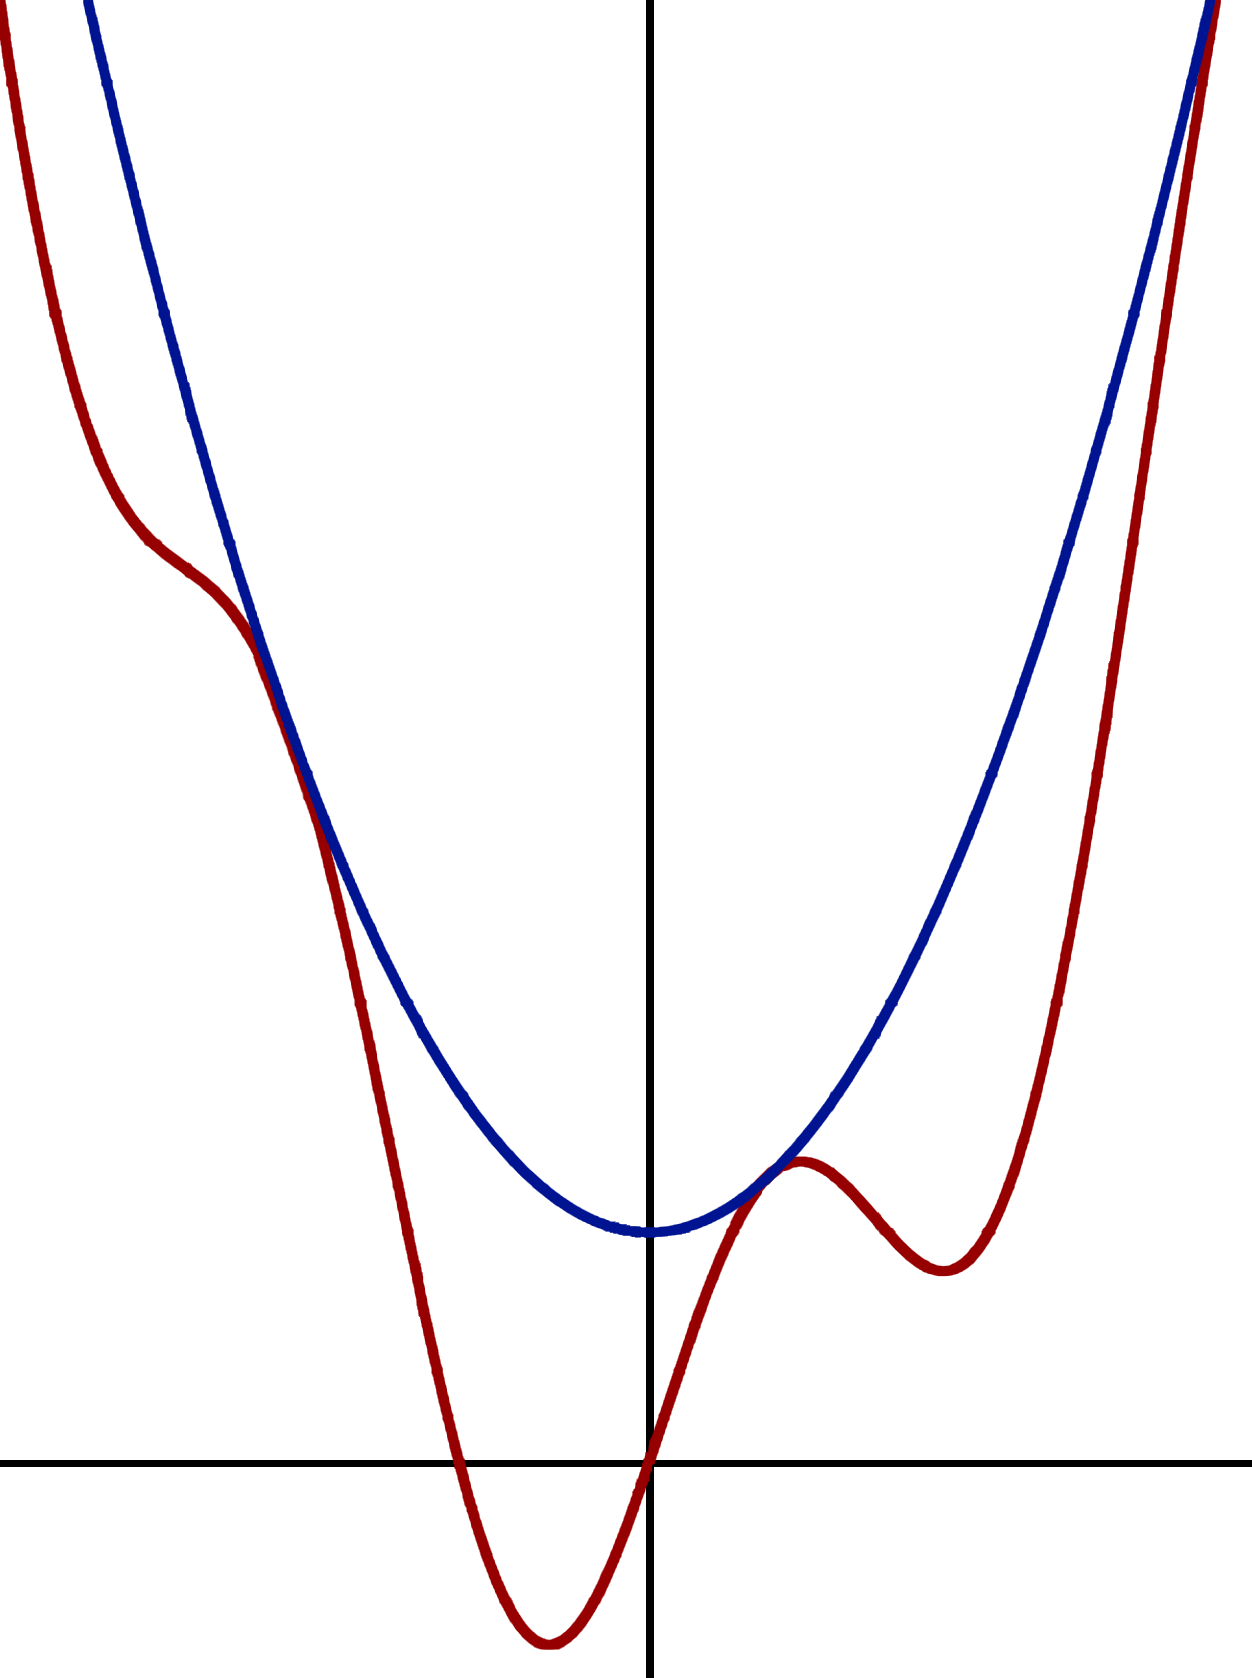
\includegraphics[width=0.3\linewidth]{Pics/PNGs/ConvexBound.png}
\end{center}
\caption{$x^2+10$ is an upper convex bound of $x^2+10sin(x)$}
\end{figure}
Accordingly, the distributed function monitoring is done on the convex bound functions, which is far simpler due to the convexity property. \\
The process of bounding a function with another convex function has to be done carefully. First, we'd like the convex bound to be $tight$, so less data is lost in the bounding process. Secondly, the state of the initial global vector has to be considered;
given a function $f$ to monitor and a starting global vector $v_0$, it's probably better to engineer a convex bound function $c$ which satisfies ${f(v_0)=c(v_0)}$. \\
After bounding the function from above and below by a convex function, the monitoring is done so whenever a local vector gets out of the convex bound, a violation is raised. The monitoring scheme tries to resolve this violation or raises a \fullSync , which updates the upper and lower convex bound functions.
In \cite{lazerson2018lightweight} the \vectorScheme \ was proposed, which resolves the violations by "balancing" the local vectors (requires high dimensional vectors to be transmitted). \\
Here, we propose the \valueScheme \ and the \distanceScheme \ which resolve the violations by sending one single scalar. Another monitoring scheme we present is the \sketchScheme \ which fuses the previously developed \vectorScheme \ and the one-dimensional schemes we developed.

%%%%%%%%%%%%%%%%% Vector Scheme %%%%%%%%%%%%%%%%%
\section{Vector Scheme}
The \vectorScheme 's main idea is to balance the server's data vectors whenever a local vector gets out of the function's convex bound. The \vectorScheme \ tries to balance the \textit{violated server} with other server's data vectors. It is done by incorporating \textit{slack vectors}, namely, $server_i$ maintains a slack $\overrightarrow{s_i}$. At all times the sum of the slacks is zero: ${\sum{\overrightarrow{s_i}} = 0}$. \\
For an upper-bound threshold, the local constraints at the servers is that ${c(v_i+s_i) > T}$. It follows that a server raises a violation and initiates a communication channel with \theCoordinator \ if ${c(v_i+s_i) > T}$, i.e. the local vector plus the slack exceeds the threshold. This ensures that whenever all the local constraint are being held, the global threshold inequality (\ref{monitoringConstraint}) is held as well.\\
Proof due to convexity of $c$, sum of slacks is zero and ${c(v_i+s_i) \leq T}$ for all $i$:
\begin{equation}
\label{vectorSchemeProof}
\begin{aligned}
 c(v)  \
	   &=  c\left(\frac{1}{n} \sum\limits_{i=0}^{n}{v_i}\right)  \
        =  \frac{1}{n} c\left(\sum\limits_{i=0}^{n}{(v_i + s_i)}\right) \\
      &\leq   \frac{1}{n} \sum\limits_{i=0}^{n}{c(v_i + s_i)}
       \leq   \frac{1}{n}(n \cdot T)
       = T
\end{aligned}
\end{equation}
When a violation occurs, and a certain server upholds ${c(v_i+s_i) > T}$, proof (\ref{vectorSchemeProof}) isn't necessarily right so a \textit{violation resolution protocol} has to be initiated.
\subsection{Violation Resolution}
In the \textit{violation resolution} phase, the slack vectors are balanced so ${c(v_i+s_i)}$ at the violated server would get inside the convex zone ${\{v \ | c(v) \leq T\}}$. When a server detects a local violation, it sends its local vector ${(v_i + s_i)}$ to \theCoordinator , which then gradually polls other servers for their local vectors. Let ${(k-1)}$ be the number of polled servers; denote ${\widetilde{v} = \frac{1}{k}\sum (v_i + s_i)}$ as the average of vectors of the polled servers and the violated server; then, whenever this average is inside the convex zone, i.e. ${c(\widetilde{v}) \leq T}$, the violation can be resolved, and no more servers have to be polled: \theCoordinator \ sends this average vector -- ${\widetilde{v}}$ to the polled servers as well as the violated server, which update their slack vector to be ${s_j \leftarrow -v_j + \widetilde{v}}$. \\
After this update, the sum of the slack vectors is still zero, and ${c(v_i+s_i) \geq T}$ at all the servers, so (\ref{vectorSchemeProof}) is correct again, and the global threshold inequality (\ref{monitoringConstraint}) holds again. \\
If all the servers are polled and still ${\widetilde{v}}$ isn't inside the convex zone ${c(\widetilde{v}) \geq T}$, a \fullSync \ has to be done; since \theCoordinator \ knows each server's ${(v_i + s_i)}$, \theCoordinator \ can calculate the global vector $v$, and hence $f(v)$. Then, the upper bound's threshold and lower bound's threshold are reset to ${(1 \pm \varepsilon )f(v)}$ and the monitoring continues with \theCoordinator \ notifying the servers of the new bounds and their local vector -- $v$ and their new slack -- the zero vector.
\subsection{Communication Bandwidth}
Considering the data vectors are of very high dimension, this scheme sends whole high dimensional vectors whenever even the slightest violation occurs. Therefore, even though the \vectorScheme \  is better than previous monitoring scheme, its still quite wasteful in communication bandwidth.

%%%%%%%%%%%%%%%%% Value Scheme %%%%%%%%%%%%%%%%%
\section{Value Scheme}
The \valueScheme \ is based on the \convexBound \ method, so it also bounds the monitored function $f$ by a convex function $c$ so it gets between the threshold and the function's value. \\ 
The \valueScheme \ is a distributed monitoring scheme which reduces the bandwidth from sending a whole high dimensional vector to sending just one scalar. The transmitted scalar represents the \textit{value} of the convex function $c$.\\
The \valueScheme \ maintains local scalar slack values; $server_i$ maintains the scalar $\lambda _i$. Also, at all times we'd enforce that the sum of the slacks is zero: ${\sum{\lambda _i} = 0}$. Here, the local server's constraint is whether ${c(v_i) + \lambda _i \leq T}$; hence, if all the local constraints are being held, the global threshold inequality (\ref{monitoringConstraint}) is held as well:
\begin{equation}
\label{valueSchemeProof}
\begin{aligned}
 c(v)  \
	    &=   c\left(\frac{1}{n} \sum\limits_{i=0}^{n}{v_i}\right)  \
       \leq   \frac{1}{n} \sum\limits_{i=0}^{n}c(v_i) \\
        &=    \frac{1}{n} \sum\limits_{i=0}^{n}{(c(v_i) + \lambda _i)}
       \leq   \frac{1}{n}(n \cdot T)
        = T
\end{aligned}
\end{equation}
When a violation occurs, i.e. ${c(v_i) + \lambda _i > T}$, proof (\ref{valueSchemeProof}) cannot longer hold, thus a violation resolution protocol has to be initiated.
\subsection{Violation Resolution}
The violation resolution protocol goes as follows: the violated server $server_i$ sends its local value ${(c(v_i) + \lambda _i})$ which exceeds the threshold $T$. \TheCoordinator \ tries to "balance" this scalar value by gradually polling other servers for their ${(c(v_i) + \lambda _i)}$ value. Let ${(k-1)}$ be the number of polled servers, then, denote ${\widetilde{\lambda} = \frac{1}{k}\sum{(c(v_i) + \lambda _i)}}$ the average of the local values plus the slacks of the polled servers and the violated server; so when ${\widetilde{\lambda} \leq T}$, the violation is resolved by sending the value $\widetilde{\lambda}$ to the polled servers and the violated server, which in turn, set their local scalar slack to ${\lambda _j \leftarrow -c(v_j) + \widetilde{\lambda} }$. Its important to note that the sum of the slacks is still zero after the resolution, and ${c(v_i) + \lambda _i \leq T}$ at all the servers as well, so proof (\ref{valueSchemeProof}) can hold again. \\
In case all the servers are being polled without being able to "balance" the slack, a \fullSync \ has to be done, which is very expensive regrading the communication bandwidth.
\subsection{Communication Bandwidth}
In the \valueScheme , the whole distributed monitoring is reduced to tracking one scalar value. Instead of transmitting a whole high dimensional vector as in the \vectorScheme , the transmitted data is just one scalar. Thus, we'd expect having much less communication bandwidth in this monitoring scheme.

%%%%%%%%%%%%%%%%% Distance Scheme %%%%%%%%%%%%%%%%%
\section{Distance Scheme}
The \distanceScheme \ is one more \textit{distributed monitoring scheme} that relies on passing a single scalar when communicating. This scheme is also based on the \convexBound \ method: the monitored function $f$ is bound by a convex function $c$ so the monitoring objective is as (\ref{monitoringConstraint}), to monitor whether ${c(v) \leq T}$. Of course, a lower-bound monitoring is done simultaneously with a different concave bound function. \\
The transmitted scalar represents the \textit{distance} to the convex function's boundary from the local vectors at the servers. \\
This scheme is based on the \distanceLemma \ which is proved below.
\subsection{The Distance Lemma}
\begin{figure}[b]
\begin{center}
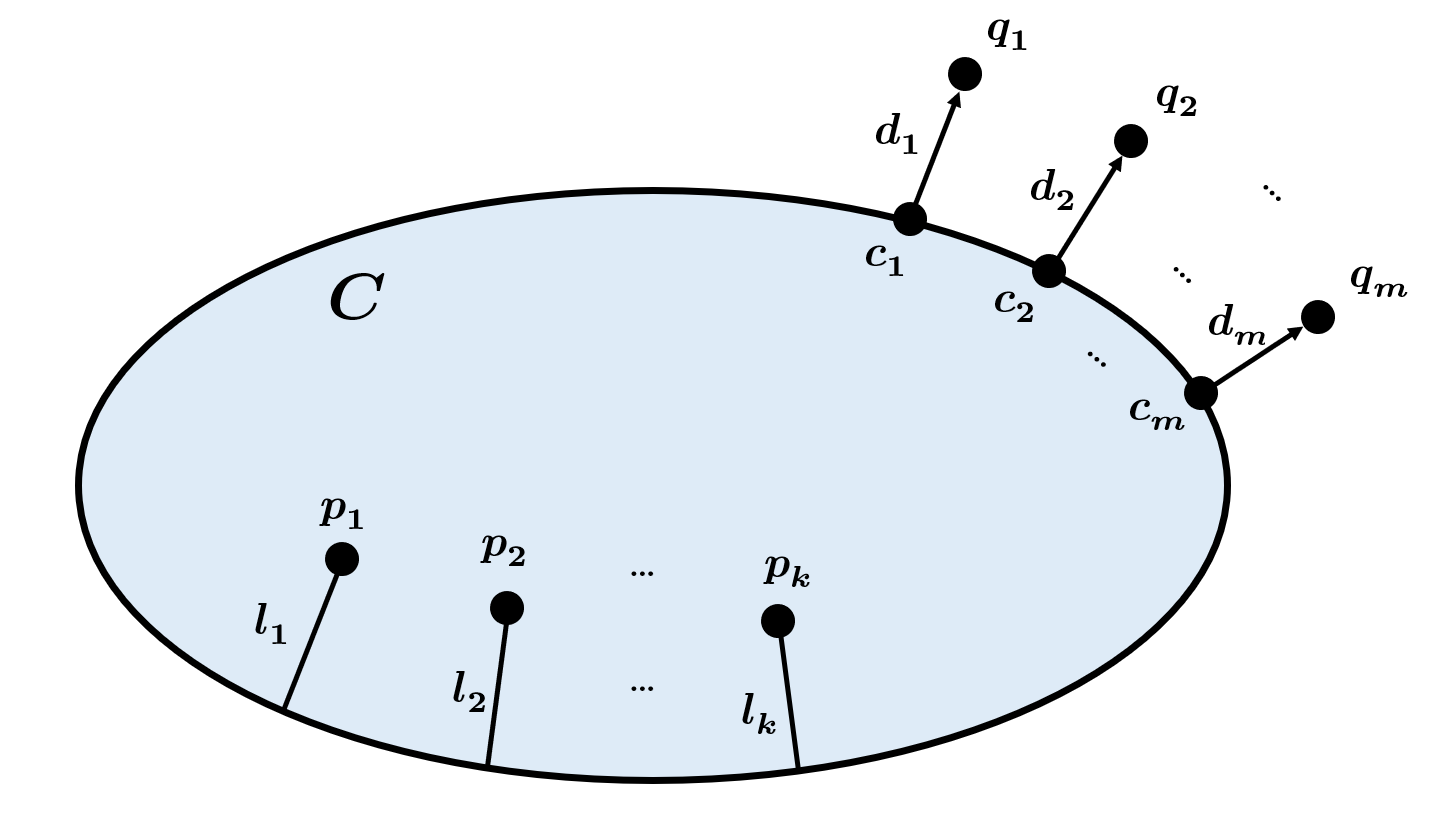
\includegraphics[width=0.9\linewidth]{Pics/PNGs/DistanceLemma.png}
\end{center}
{\centering
\caption{The \distanceLemma}}
\medskip
\small
The average of ${p1...p_k, q_1...q_m}$ is inside the convex body $C$ if ${\sum l_i \geq \sum ||d_i||}$.
\end{figure}
The \distanceLemma \ states that the average of points is inside a convex body, if the sum of the distances to the surface of the points inside the convex body is greater than the sum of the distances to the boundary of the points outside of the convex body. This \distanceLemma \ is the basis of the \distanceScheme . \\

The \distanceLemma : Let ${\{v_1 ... v_n\}}$ be vectors and let $C$ be a convex body. If the sum of the distances to the boundary of $C$ of the vectors inside $C$ is greater than the sum of the distances to the boundary of the vectors from outside, then the average vector ${\frac{1}{n}\sum {v_i}}$ is inside the convex body. \\
proof: \\
\begin{enumerate}
\item Let ${p_1 ,..., p_k}$ be the points inside the convex body $C$ and ${l_1 ,..., l_k}$ their distances to the boundary.
\item Let ${q_1 ,..., q_m}$ be the points outside the convex body $C$ and ${d_1 ,..., d_m}$ the distance vectors from the boundary to the points. Let ${c_1 ,..., c_m}$ be the points on the boundary which are the sources of the distance vectors ${d_1 ,..., d_m}$ respectively.
\item Let ${d = \sum {d_i}}$ and ${l = \sum {l_i}}$
\item Assume $l \geq \sum ||d_i||$, so $l \geq ||d||$
\item It's needed to prove that the average point is inside the convex body, i.e., prove that ${\frac{1}{k+m}(\sum{p_i} + \sum{q_i}) \in C}$:
\end{enumerate}
\begin{equation}
\begin{aligned}
&( p_1+...+p_k) + (q_1+...+q_m) = \\
&( p_1+...+p_k) + (c_1+d_1) + ... + (c_m + d_m) = \\
&( p_1+...+p_k) + d + (c_1 + ... + c_m) = \\
&\left( p_1 + \frac{l_1 d}{l}\right) + ... + \left(p_k + \frac{l_k d}{l}\right) + (c_1 + ... + c_m)
\end{aligned}
\end{equation}
\begin{enumerate}
\item[\ \ \ ] ${c_i \in C}$ by definition -- $c_i$ is on the boundary of $C$. Also, ${p_i + \frac{l_i d}{l} \in C}$ because ${l \geq ||d||}$ and $l_i$ is the distance of $p_i$ to the boundary. \\
Since an average of points inside a convex body is also inside the convex body, ${\frac{1}{k+m}(\sum{p_i} + \sum{q_i}) \in C \ \blacksquare} $ 
\end{enumerate}
\subsection{Distributed Monitoring}
The \distanceScheme 's monitoring is based on the distance value of the local vectors to the function's convex bound geometric boundary. The \distanceScheme \ literally monitors distributively whether the sum of the distances from inside to the boundary is greater than the sum of the distances to the boundary from the outside. For convenience, denote the distance to the boundary from inside the convex body as negative, and the distance from outside as positive, therefore, the \distanceScheme \ monitors whether the sum of the distances is negative. \\
Like the \valueScheme , the \distanceScheme \ maintains slack scalars that would help "balance" the distances from the boundary between servers as the data changes. Let $server_i$ maintain the scalar $\lambda _i$. As in \valueScheme , at all times the sum of the slacks is zero: ${\sum {\lambda _i} = 0}$. \\
Denote $d_i$ the distance of $server_i$'s vector to the boundary, then the local server's monitoring constraint is whether ${d_i + \lambda_i \leq 0}$. Therefore, if all the local constraints hold, the global vector's distance is negative and by the \distanceLemma , the global threshold inequality (\ref{monitoringConstraint}) holds:
\begin{equation}
\label{distanceSchemeProof}
\sum{d_i} = \sum{(d_i + \lambda _i)} \leq n \cdot 0 = 0
\end{equation}
The sum of the distances is negative, thus the average vector is inside the convex safe zone ${\{v \ | \ c(v) \leq T \}}$. \\
Whenever ${d_i + \lambda _i > 0}$ at a certain server, a violation occurs and a  \textit{violation resolution protocol} begins. 
\subsection{Violation Resolution}
When the local vector at a server changes so ${d_i + \lambda _i > 0}$, a violation occurs. In order to resolve the violation, the $\lambda _i$ slacks has to be "balanced" so ${d_i + \lambda _i \leq 0}$ at the violated server as well as other servers where some slack would be "borrowed". \\
Firstly, in order to resolve the violation, the violated server sends its ${(d_i + \lambda _i)}$ value to the \Coordinator ; afterwards, \theCoordinator \ gradually polls other servers for their ${(d_i + \lambda _i)}$ value. Let $(k-1)$ be the number of polled servers, denote ${\widetilde{\lambda} = \frac{1}{k}\sum(d_i + \lambda _i)}$ the average of distances plus the slacks of the polled servers and the violated server; then when ${\widetilde{\lambda} \leq 0}$, the violation can be resolved: \theCoordinator \ sends the single value $\widetilde{\lambda}$ to the polled servers and the violated server, where they update their slacks so ${\lambda _j 
\leftarrow -d_j + \widetilde{\lambda}}$. Note that the sum of slacks is still zero after the update, and at each server the local constraint holds, ${d_i + \lambda _i \leq 0}$, so proof (\ref{distanceSchemeProof}) holds again.
\subsection{Communication Bandwidth}
The monitoring is done solely by the value of the distance. A scalar value is transmitted between the \Coordinator \ and the servers, thus we'd expect much less communication bandwidth than the \vectorScheme .

%%%%%%%%%%%%%%%%% Value Scheme vs. Distance Scheme %%%%%%%%%%%%%%%%%
\section{Value Scheme vs. Distance Scheme}

\begin{figure}[t]
\begin{center}
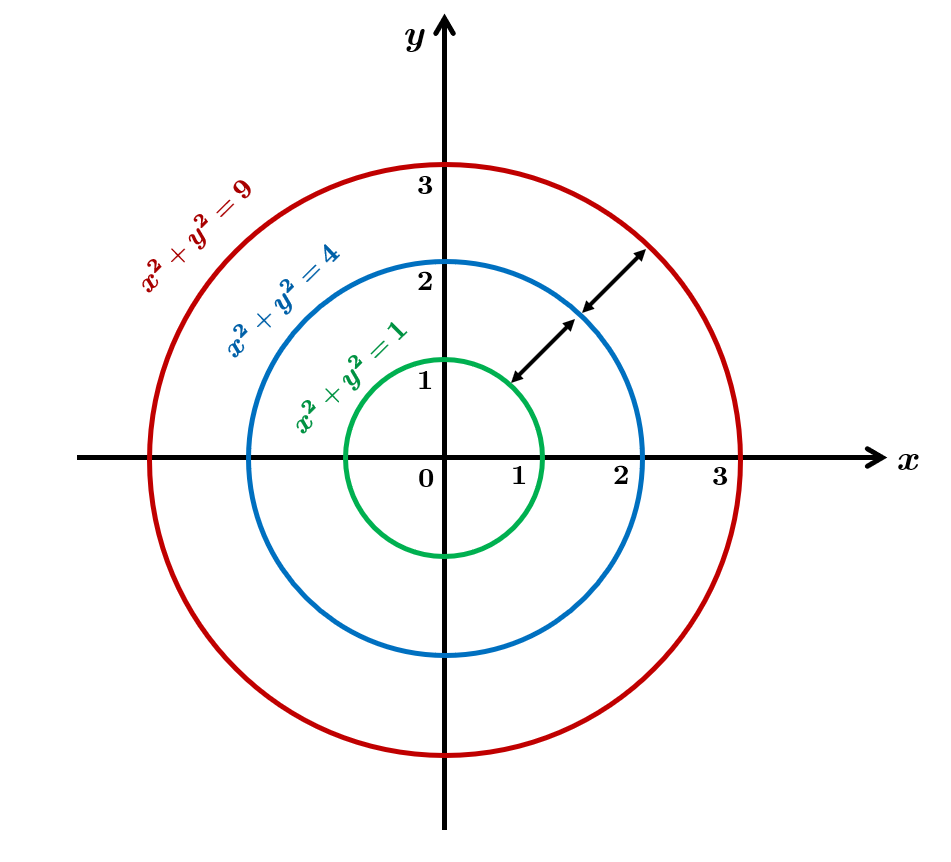
\includegraphics[width=\linewidth]{Pics/PNGs/L2NormDistanceVsValue.png}
\end{center}
\caption{Norm $L2$ Squared distance and value behaviour}
\label{fig:L2NormDistanceVsValue}
\medskip
\small
The value of the function $||v||^2$ quadratically grows in relation to the distance.
\end{figure}

\begin{figure*}[t]
\begin{minipage}[t]{0.49\linewidth}
{\centering
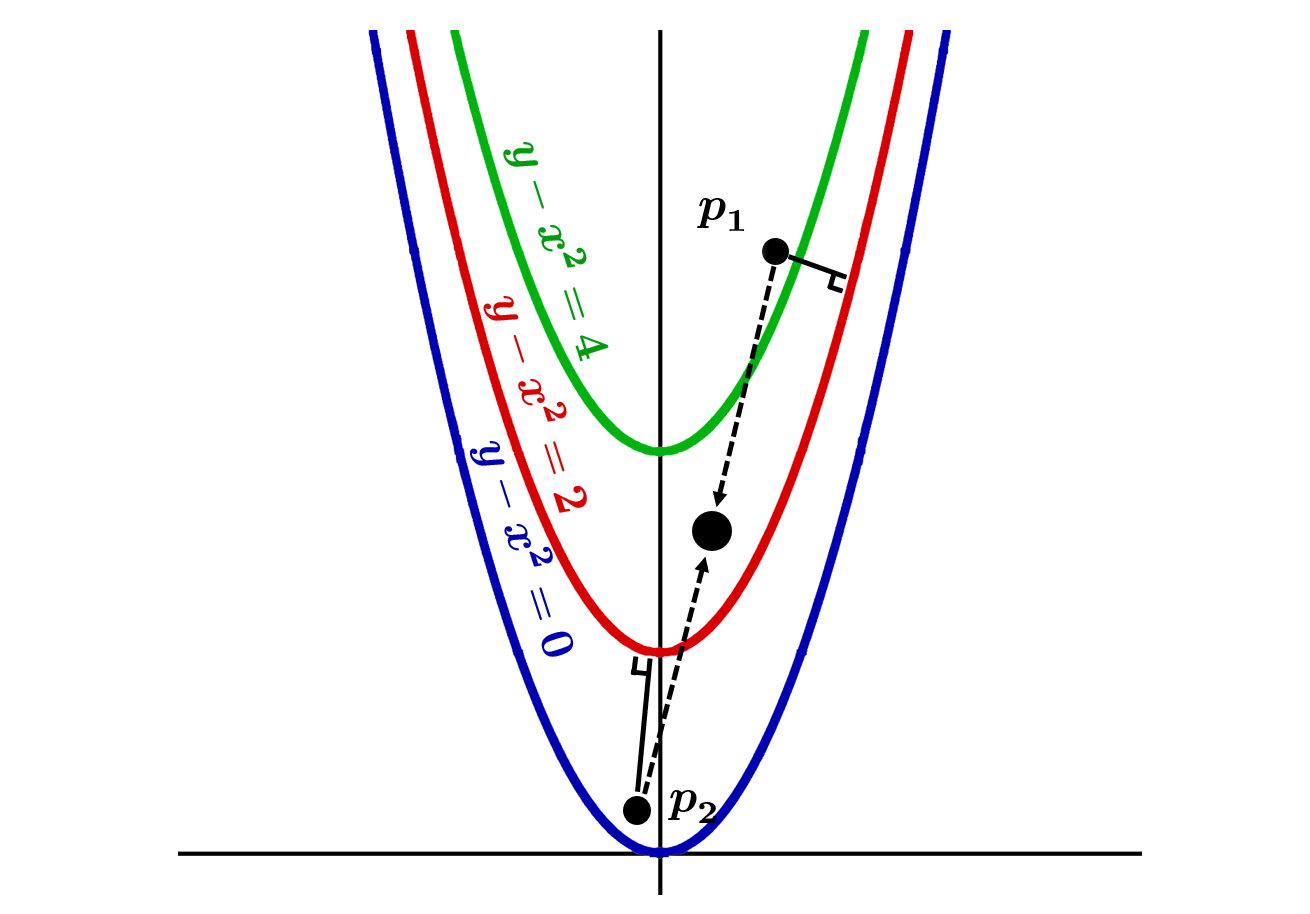
\includegraphics[width=\textwidth]{Pics/PNGs/ValueSchemeBetter.png}
\caption{\valueScheme \ beats \distanceScheme}
\label{fig:valueBeatsDistanceFigure}}
\medskip
\small
When monitoring ${y-x^2 \geq 2}$, the distance to the boundary ${f(x, y) = y - x^2 = 2}$ from the outside point $p_2$ is greater than the distance from the inside point -- $p_1$, though ${\frac{1}{2}(f(p_1)+f(p_2))\geq 2}$, so the \valueScheme \ won't raise a violation, while the \distanceScheme \ will raise a violation which is a \falseAlarm .

\end{minipage}
\begin{minipage}[t]{0.02\linewidth}
\hfill
\end{minipage}
\begin{minipage}[t]{0.49\linewidth}
{\centering
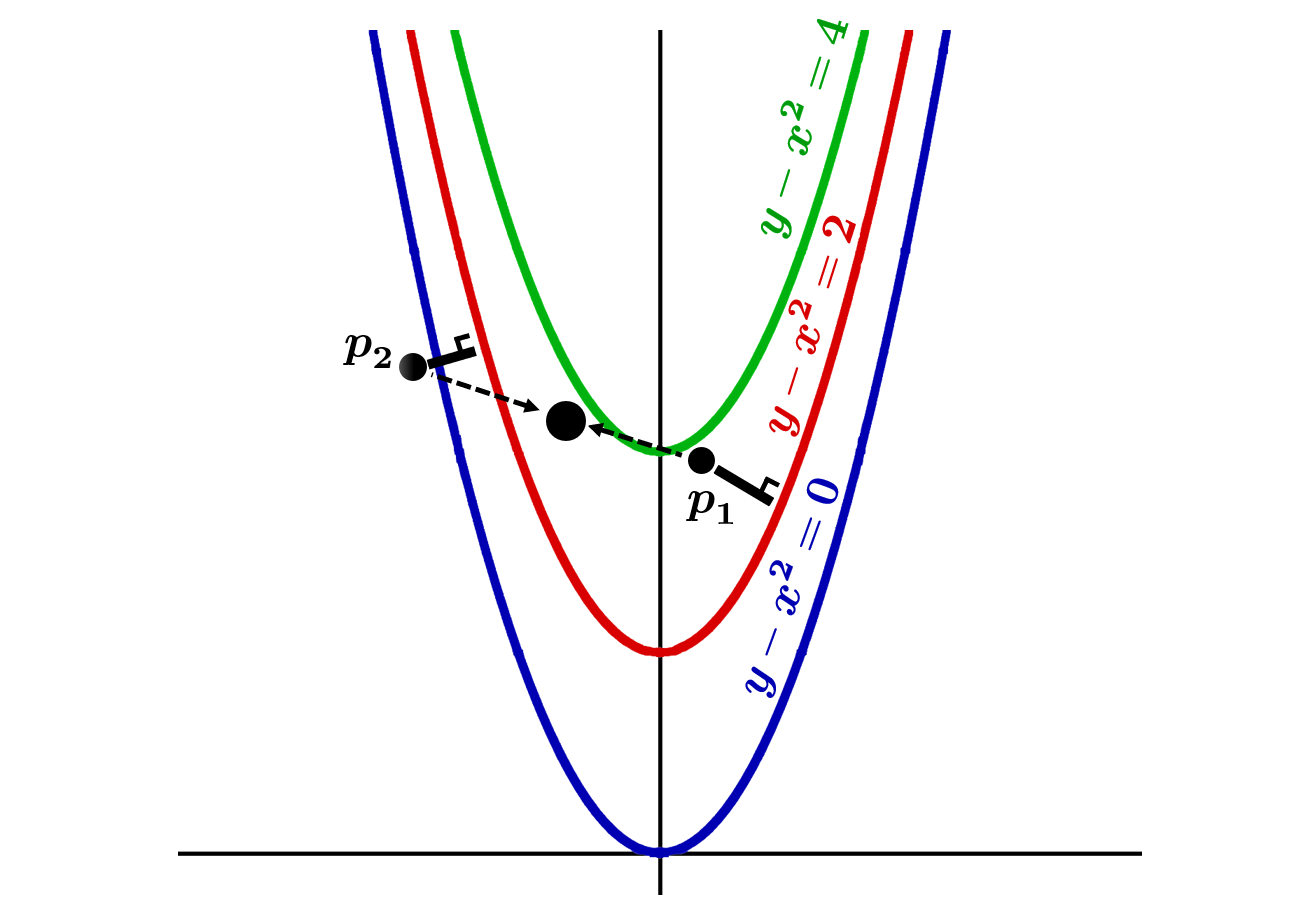
\includegraphics[width=\textwidth]{Pics/PNGs/DistanceSchemeBetter.png}
\caption{\distanceScheme \ beats \valueScheme}
\label{fig:distanceBeatsValueFigure}}
\medskip
\small
When monitoring ${y-x^2 \geq 2}$, the distance to the boundary ${f(x,y) = y - x^2 = 2}$ of the inside point $p_1$ is greater than the distance of the outside point $p_2$, however, ${\frac{1}{2}(f(p_1)+f(p_2))< 2}$, so the \valueScheme \ will raise a false-negative violation, while the \distanceScheme \ correctly won't raise a violation.
\end{minipage}
\end{figure*}

Both \valueScheme \ and \distanceScheme \ are distributed monitoring schemes which are reduced to tracking just one scalar value. In the \distanceScheme \ its the sum of the distances to the convex bound's geometric boundary, and in the \valueScheme \ its the average of the convex function's value. \\
A good question that arises is which monitoring scheme is better? which one uses less communication bandwidth? Is there a connection between the schemes? \\
In [*] its proposed there's a linear correlation between the distance to the geometric representation of a function and the value of the function when the distance is small. Hence, we'd expect similar results of the schemes. \\
Nonetheless, since we deal with convex functions, the value grows faster than the function's distance. A good example is the function ${f(x) = x^{100}}$ which  when monitoring ${f(x) \leq 1}$, the function's value changes rapidly outside the boundary as $x$ changes a bit; so the distance changes much slower than the value. Accordingly, we'd expect the \distanceScheme \ to be better on those convex function whose value grows rapidly in relation to the distance (vice versa cannot occur since the function is convex). This behaviour is shown in the experiment done in subsection \ref{L2SquaredExperiment} on the function ${f(v) = ||v||^2}$, where \distanceScheme 's communication bandwidth is much less than the \valueScheme . The quadric relation of the value-distance is demonstrated in Fig. \ref{fig:L2NormDistanceVsValue}. \\
Even though in convex functions the growth of the distance progresses slower than its value, it doesn't necessarily imply that the distance scheme is better. The function's value growth is two sided -- when a function grows fast on one direction, it may decay fast on the reverse direction. For example, when monitoring the convex condition ${f(x) = y-x^2 \geq 2}$, the results aren't conclusive. As shown in Fig. \ref{fig:valueBeatsDistanceFigure} and Fig. \ref{fig:distanceBeatsValueFigure}, there are cases of false negative violations which occur only in one distributed monitoring scheme and not the other; the global average vector remains inside the convex bound ${f(x) \geq 2}$ while a false alarm can be raised. \\
Another important factor is that the \valueScheme \ is computationally mathematically whole, while the \distanceScheme \ may require some approximations; the problem of finding the distance to a convex surface from outside is mathematically closed using convex optimization techniques \cite{boyd2004convex}. On the other hand, finding the distance from inside to the convex surface isn't always solvable [**], so unfortunately the \distanceScheme \ isn't applicable on all possible functions that require distributed monitoring.

%%%%%%%%%%%%%%%%% Data Resolution %%%%%%%%%%%%%%%%%
\section{Sketched Data Scheme}
The \sketchScheme \ is a gradual integration of the \vectorScheme \ and either the \valueScheme \ or the \distanceScheme . \\
This scheme behaves like the \valueScheme \ or the \distanceScheme \ up until a violation which cannot be resolved occurs and a \fullSync \ has to be done. Instead of a \fullSync , \theCoordinator \ polls the servers for a \textit{sketch}, i.e., a lossy compression of their change vector of the data; the average of the sketches is combined and sent to the servers, which infer some information from it which might help continuing the monitoring without invoking an expensive \fullSync. For the sketch function, multiple functions can be used, such as sending the most dominant elements of the change-vector, the most dominant DCT parameters of the change-vector and the most dominant PCA parameters etc. \\
The better the sketch represents the change vector, the more beneficial information the servers will deduce which will help overcome the violation that occurred in the one-dimensional scheme (\valueScheme \ or \distanceScheme ). \\
Practically, the \sketchScheme \ performs a softer more gradual \fullSync; if this partial \fullSync \ still won't allow the one-dimensional distributed monitoring scheme to be continued, the dimension of the sketch will be raised so the lossy compressed sketches would be more representative of the global vector, hopefully allowing the one dimensional scheme to continue. \\
\subsection{Distributed Monitoring}
The algorithm of the \sketchScheme \ acts as follows:
\begin{enumerate}
\item Choose a one-dimensional distributed monitoring scheme (\valueScheme \ or \distanceScheme ), note it $\sigma$.
\item \label{OneDimensionalMonitoring} Distributively monitor the global monitored function according to $\sigma$.
\item \label{ResolutionAfterFullSync} When a \fullSync \ has to be invoked because of $\sigma$, each server sends a sketch of dimension $d$ of the change vector to \theCoordinator . Initially $d = const$.
\item \TheCoordinator \ sends the average of the sketches to the servers in a compressed form according to the sketch function.
\item The servers add the average of sketches to their reference vector, and set their change vector to be the "error" of their compression over their original change vector.
\item Try continuing monitoring by $\sigma$, if it doesn't immediately raise a \fullSync \ -- set ${d = const}$ and go to (\ref{OneDimensionalMonitoring}) to continue monitoring. \\
Otherwise, if a \fullSync \ was raised immediately, multiply $d$ by two, and go to (\ref{ResolutionAfterFullSync}) to try resolving the violation.
\item If $d$ reaches the value of quarter of the data-vector dimension, invoke a global \fullSync , set $d = const$ and go to (\ref{OneDimensionalMonitoring}) to continue monitoring.
\end{enumerate}
\subsection{Violation Resolution}
Here we'll elaborate about the violation resolution phase of the \sketchScheme . The violation resolution of the \sketchScheme \ is invoked when the one-dimensional monitoring scheme fails. 
\begin{enumerate}
\item Let $n$ be the number of servers. Let $r_0$ be their reference vector and $ch_1 ... ch_n$ be their data's change-vectors of the servers.
\item Let $d$ be the chosen dimension of the violation resolution.
\item Let $sk_d$ be a lossy sketch function of dimension $d$. Let $sk_d (ch_i)$ be the sketch of the change vector of the i-th server, and $\varepsilon _d(ch_i)$ be the "error" of the sketch function so ${ch_i = sk_d(ch_i) + \varepsilon _i(ch_i)}$ for all $server_i$.
\item Each server sends its $sk_d(ch_i)$ to \theCoordinator \ in a compressed form.
\item \TheCoordinator \ calculates the average of the sent vectors ${\widetilde{sk_d} = \frac{1}{n}\sum sk_d(ch_i)}$ and transmits it to the servers.
\item Each server $server_j$ updates its reference vector to be ${r_0 \leftarrow r_0 + \widetilde{sk_d}}$. The change vectors are updated as well: ${ch_j \leftarrow \varepsilon _j(ch_j)}$.
\item Try continuing the one-dimensional distributed scheme.
\item If the one-dimensional scheme immediately tries to invoke a \fullSync \ again, raise the sketch dimension to $2\cdot d$ up to $\frac{n}{4}$.
\item If a violation reoccurs when ${d > \frac{n}{4}}$ invoke a \fullSync .
\end{enumerate} 
It's important to note that at all times before and after the violation, the global vector remains the same: ${v = \frac{1}{n}\sum v_i=\frac{1}{n}\sum (r_0 + ch_i)}$. Moreover, the "error" of the sketch function is taken into account so there's no probabilistic nature to this scheme. The more the sketch function represents the change vector, the  better the local vectors of the servers estimate the global vector.
\subsection{Communication Bandwidth}
The \sketchScheme \ actually makes the \fullSync \ more gradual. Instead of sending the whole data vectors, it sends it bit by bit, so when the partially average vector is enough for the \valueScheme \ or the \distanceScheme \ to continue monitoring on its own -- there's no need for more communication to be made. \\
In addition, the sketches are done on the change vector, so the servers embed the data they get from round to round into the reference vector, hence the "information" the server receives gets accumulated; therefore, when a \fullSync \ has to be invoked, already half of the global change vector is accumulated by the servers, so what's left is only the other half, which make the \fullSync \ more efficient, requiring half as much communication bandwidth. \\
Also, since the dimension of the sent vector doubles itself from round to round, the latency of the \sketchScheme \ is logarithmic to the dimension of the data.  

%%%%%%%%%%%%%%%%% Experimental Results %%%%%%%%%%%%%%%%%
\section{Experimental Results}
In order to assess the productivity of the distributed monitoring schemes proposed, we tested the communication bandwidth of the data sent between the servers and \theCoordinator \ both on real-world diverse data and synthetic scheme-oriented data. \\
As for the distributed dynamic monitored data, we used a bag-of-words vector of high dimension constructed of occurrences of tokens at a moving sliding window. \\
The servers data is diverse: one is created out of blogs from \textit{bloggers.com} while other is fed of tweets posted online, other from Amazon reviews, one more from Reddit comments etc.
\subsection{Oracle Scheme and Naive Scheme}
One of the needs of comparing between the monitoring schemes and assessing whether the monitoring schemes proposed really are economical bandwidth-wise, is offering a lower bound and an upper bound for distributed monitoring schemes. \\
The obvious communication-bandwidth upper bound is the \naiveScheme \ which simply sends each data change at a server to \theCoordinator , so virtually, the global vector is known, and the computation isn't distributed but centralized. This method obviously isn't very bandwidth efficient, though its a good upper bound for comparison. \\
For the lower bound of the communication bandwidth, we propose the \oracleScheme \ which is like an oracle who does not have false negative violations. Simply, no communication is done, apart from whenever a \textit{true violation} occurs and a \fullSync \ is invoked. Let $\mu$ be the last "known" value of $f(v)$, then, a \textit{true violation} is when ${f(v) > (1
+\varepsilon)\mu}$ or ${f(v) < (1-\varepsilon)\mu}$ (for simplicity, assume ${\mu \geq 0}$). Naturally, all the changed data  is sent at a \fullSync , and the value of $\mu$ is updated as well as the thresholds values. \\
In other words, \oracleScheme \ transmits data only when it's truly needed to be passed -- when a \fullSync \ must be done. \\
Of course this scheme isn't realistic, since a server knows nothing about its neighbours, so the global vector isn't known. False violation obviously have to occur from time to time. 
\subsection{Norm $L_2$ Squared} \label{L2SquaredExperiment}
\begin{figure}[t]
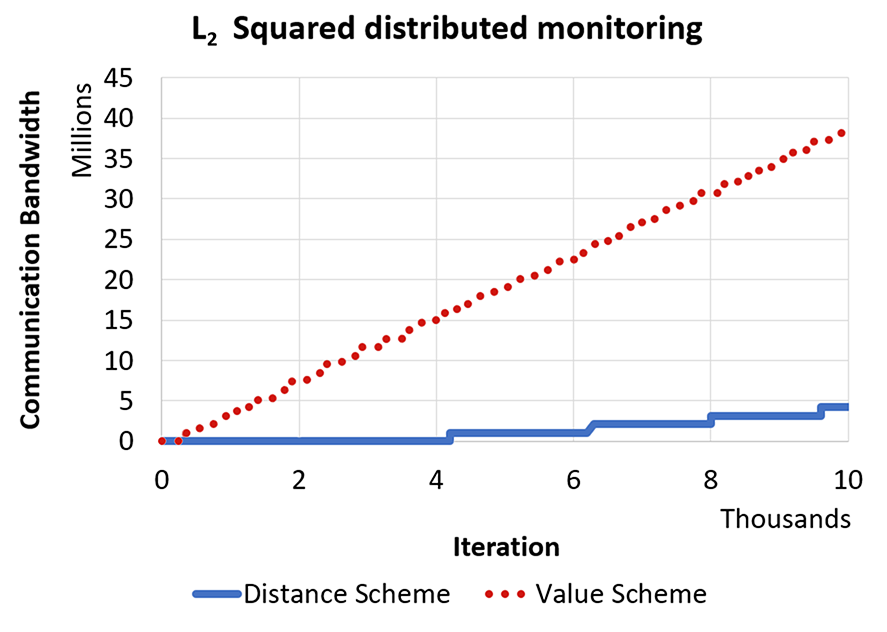
\includegraphics[width=\linewidth]{Pics/PNGs/L2NormCommunicationDiagram.png}
\caption{Distributed Monitoring of the $L_2$ Squared Function}
\medskip
\small
\distanceScheme \ uses much less communication bandwidth than \valueScheme \ when monitoring norm $L_2$ squared function.
\label{SphereMonitoring}
\end{figure} 
The $L_2$ norm is widely used in multiple scenarios, either for (...) [*] or for (...) [**]. \\
Here, we monitored the $L_2$ norm squared, namely ${f(v) = ||v||^2}$. One of the reasons is to confirm that this function requires less communication bandwidth using the \distanceScheme \ in contrast to the \valueScheme . \\
\subsubsection{Lower and Upper Bounds}
Finding the convex bound of the function isn't difficult since it's convex; the upper bound is the function itself, and the lower bound's concave function is the tangent plane to the function at the closest point from the global vector. Computing the distance from a point to the boundary also is fairly easy -- both to the sphere and to the tangent plane. \\
\subsubsection{Experiments}
In order to check the difference between the \valueScheme \ and the \distanceScheme \ we constructed one hundred servers with dynamic vectors in dimension $\num[group-separator={,}]{10000}$. The changes were of small steps in all the $\num[group-separator={,}]{10000}$ dimensions. \\
The bandwidth results over time are presented in Fig. \ref{SphereMonitoring}. The \distanceScheme \ resulted in about eight times less transmitted data. \\
Since we started with zero vectors, we monitored the function by bounding it additively ${(\pm 10)}$ instead of a multiplicative ${(1 \pm \varepsilon)}$.

\subsection{Entropy}
\begin{figure}[b]
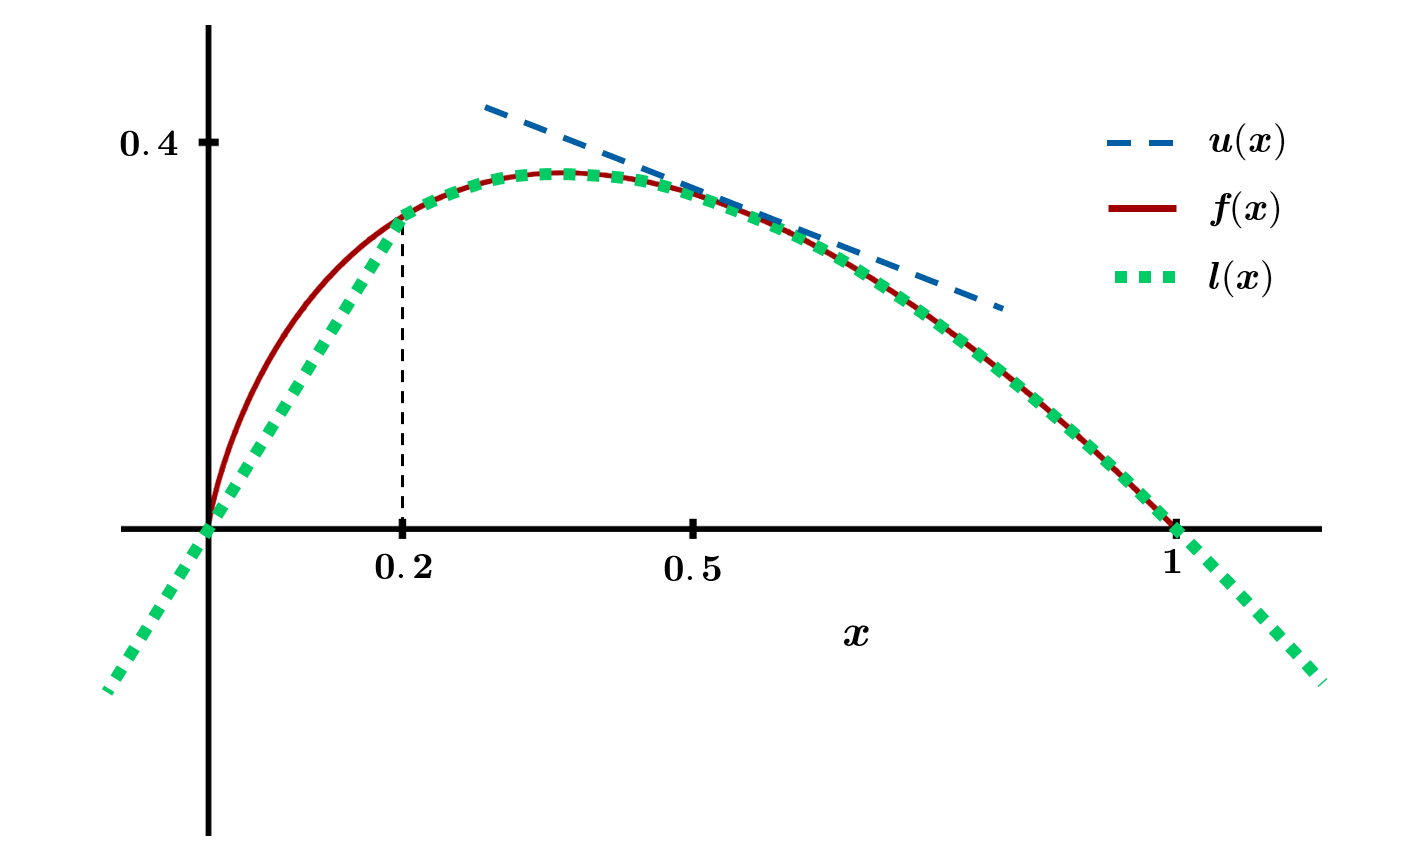
\includegraphics[width=0.85\linewidth]{Pics/PNGs/EntropyBounds.png}
\caption{Entropy Function's Upper and Lower Bounds}
\label{EntropyBoundsFigure}
\medskip
\small
${f(x) = -xln(x)}$ is the entropy function. A convex upper bound is the tangent plane at a point as in $u(x)$. A concave lower bound is shown in $l(x)$. The extension point $p_0 = 0.2$ is chosen for illustration.
\end{figure}
The Entropy function is widely used in computer science applications. Whether its tracking a distributed denial of service attack and network anomalies \cite{arackaparambil2010distributed}, medicine applications \cite{anderson2004entropy} or detection of physical activity using wearable sensors \cite{ermes2008detection}. \\
The entropy function of the probability-vector $v$ of dimension $n$ is defined as follows:
\begin{equation}
f(v) = f(v_1,...,v_n)=\sum\limits_{i=0}^n -v_i \cdot ln(v_i)
\end{equation}
\subsubsection{Lower and Upper Bounds}
Applying the convex-bound method on the entropy function requires finding a convex bound from above and a concave bound from below. As for the upper bound, since the function is concave, a good upper bound is the tangent plane at the closest point. For the lower bound, seemingly, because the function is concave, it should be its own concave bound, which isn't fully correct. Notice we work not on the data vectors but on  the reference point plus the change vector, so parameters can become negative, which isn't defined on the entropy function. Consequently, we'd have to "extend" the entropy function to the negative part. As  suggested in \cite{gabel2017anarchists}, we bound the entropy function by itself, but below the point where the probability is $p_0 = \frac{1}{const}$ we take the line that starts at $p_0$ and passes at the origin of the coordinate system. A sketch of an instance of an upper bound and lower bound of the entropy function is shown in Fig. \ref{EntropyBoundsFigure}. \\
After finding the convex upper bound and the lower concave bound, distributed monitoring of the entropy can be done by applying the \valueScheme \ or the \vectorScheme \ , though the \distanceScheme \ requires being able to calculate distances to the bounding function's surface. \\
\subsubsection{Distance to Bounds}
The main challenge is computing the distance from inside the concave lower bound.  \\
The convex upper bound is a tangent plane. Finding the distance from a point to the tangent plane's surface has a closed mathematical solution. \\
As for the concave lower bound, finding the distance to the entropy's bound surface from outside is solvable by convex optimization \cite{boyd2004convex}, but from inside, finding the $L_2$ norm isn't easy. So instead of computing the $L_2$ distances, we compute $L_1$ distances so the \distanceScheme \ is done on $L_1$ distances. Note that the \distanceLemma \ is correct on any norm of distances since the norm it uses requires only the triangle inequality. \\
Since the entropy's lower bound function is concave and permutation invariant, finding its $L_1$ distance can be calculated by a basic binary search on the value of $L_1$ done by climbing the derivation function. \\
Unfortunately, this method for finding the $L_1$ distance to the surface is quite costly in time for high dimensional vectors, thus allowing us to experiment only on low dimensional data using the \distanceScheme .
\subsubsection{Experiments}
.... \\
\subsection{Inner Product}
In order to adjust the inner-product function to the distributed monitoring model, we treat the inner-product as a function whose input is a vector of even dimensionality. Denote ${[x \circ y]}$ as the concatenation of vectors $x$ and $y$. Assume $x$ and $y$ are of the same dimensionality, then the inner product function is defined as follows:
\begin{equation}
f([x \circ y]) = <x, y>
\end{equation}
The inner-product function is extensively used in mathematics and computer science either as a similarity measure of data [*] or as a basic component of other functions: it's used in data mining applications [*] and machine learning softwares [*] and also in ... [*]. \\
\subsubsection{Lower and Upper Bounds}
A good trick presented in \cite{lazerson2015monitoring} is representing a function as a difference of two convex functions, ${f(v) = c_1(v)-c_2(v)}$; then, binding it by a convex (concave) function requires solely bounding the negative (positive) part from above (below) by a tangent plane. \\
As for the inner product, it upholds that ${<x,y> \ = \ 0.25(||x+y||^2-||x-y||^2)}$ which is a difference of two convex functions. \\
\subsubsection{Distance to Bounds}
After having a closed mathematical representation to the upper and lower bound, the distance from a point to the function's surface can be found using the method of Lagrange multipliers which yield a closed mathematical solution. \\
\subsubsection{Experiments}
....

%%%%%%%%%%%%%%%%% Conclusions %%%%%%%%%%%%%%%%%
\section{Conclusions}
....

%%%%%%%%%%%%%%%%% References %%%%%%%%%%%%%%%%%
\bibliographystyle{ieeetran}
\bibliography{References}

%%%%%%%%%%%%%%%%% End Document %%%%%%%%%%%%%%%%%
\end{document}
